
\begin{ex}%[Nguồn: Bộ đề minh họa Moon 2024-2025]%[2P6V3-5]%
	Trong không gian với hệ tọa độ $Oxyz$, cho điểm $E(1;1;1)$, mặt cầu $(S)\colon x^2 + y^2 + z^2 = 4$ và mặt phẳng $(P)\colon x - 3y + 5z - 3 = 0$. Gọi $\Delta$ là đường thẳng đi qua $E$, nằm trong $(P)$ và cắt mặt cầu $(S)$ tại hai điểm $A$, $B$ sao cho tam giác $OAB$ là tam giác đều. Đường thẳng $\Delta$ có một vectơ chỉ phương là $(a; b; 10)$. Tính $a^2 + b^2$.
	\shortans[oly]{$6500$}
	\loigiai{
	\begin{itemize}
		\item Mặt phẳng $(P)$ có VTPT là $\overrightarrow{n}=(1;-3;5)$. \\
		Đường thẳng $\Delta$ có VTCP là $\overrightarrow{a}=(a;b;10)$.\\
		Đường thẳng $\Delta$ nằm trong $(P)$ nên $\overrightarrow{n}\cdot\overrightarrow{a}=0\Leftrightarrow a-3b+50=0\Leftrightarrow a=3b-50$.\\
		Hay $\overrightarrow{a}=(3b-50;b;10)$.
		\item Mặt cầu $(S)$ có tâm $O(0;0;0)$ và bán kính $R=2$.\\
		Gọi $M$ là trung điểm của $AB$, do $\triangle OAB$ là tam giác đều nên $OM=\dfrac{OA\sqrt{3}}{2}=\sqrt{3}$.\\
		Gọi $d$ là khoảng cách từ tâm $O$ đến $\Delta$ thì $d=OM=\sqrt{3}$.
		\item Mặt khác, $d=\dfrac{\big|[\overrightarrow{a},\overrightarrow{OE}]\big|}{\big|\overrightarrow{a}\big|}=\sqrt{\dfrac{14b^2-780b+6200}{10b^2-300b+2600}}$.
		\item Do đó
		\allowdisplaybreaks
		\begin{eqnarray*}
			&&\sqrt{\dfrac{14b^2-580b+6200}{10b^2-300b+2600}}=\sqrt{3}\Leftrightarrow\dfrac{14b^2-780b+6200}{10b^2-300b+2600}=3\\&\Leftrightarrow&14b^2-580b+6200=3(10b^2-300b+2600)\\
			&\Leftrightarrow&16b^2-320b+1600=0\Leftrightarrow b=-10.
		\end{eqnarray*}
		Khi đó $a=-80$.\\
		Vậy $a^2+b^2=(-80)^2+(-10)^2=6500$.
		
	\end{itemize}
	}
\end{ex}

\begin{ex}%[Nguồn: Bộ đề minh họa Moon 2024-2025]%[1C2H3-1]
	Có $4$ người và $1$ đèn pin muốn qua sông phải đi qua một cây cầu. Biết cây cầu chỉ đi $1$ lần tối đa được $2$ người và phải có đèn pin mới có thể di chuyển trên cầu. $A$ đi qua cầu hết $1$ phút, $B$ hết $2$ phút, $C$ hết $5$ phút, $D$ hết $10$ phút. Hai người đi cùng nhau thì phải đi với tốc độ của người đi chậm hơn. Hỏi mất ít nhất bao nhiêu phút để tất cả đều qua được sông?
	\shortans[]{$17$}
	\loigiai{
	Để tối ưu hóa thời gian ta qua cầu sẽ có xu hướng xếp hai người đi chậm nhất là $C$ và $D$ cùng qua cầu một lượt. Ta có cách sắp xếp sau
	\begin{itemize}
		\item Lượt 1. $A$ và $B$ cùng qua cầu hết $2$ phút.
		\item Lượt 2. $A$ quay lại hết $1$ phút.
		\item Lượt 3. $C$ và $D$ cùng qua cầu hết $10$ phút.
		\item Lượt 4. $B$ quay lại hết $2$ phút.
		\item Lượt 5. $A$ và $B$ cùng qua cầu hết $2$ phút.
	\end{itemize}
	Vậy tổng thời gian ngắn nhất để cả bốn người qua cầu là $17$ phút.
	}
\end{ex}

\begin{ex}%[Nguồn: Bộ đề minh họa Moon 2024-2025]%[2P1V7-9]
	[TL.309840]
	Theo thống kê tại một nhà máy Z, nếu áp dụng tuần làm việc $40$ giờ thì mỗi tuần có $100$ công nhân đi làm và mỗi công nhân làm được $120$ sản phẩm trong một giờ. Nếu tăng thời gian làm việc thêm $2$ giờ mỗi tuần thì sẽ có $1$ công nhân nghỉ việc và năng suất lao động giảm đi $5$ sản phẩm/$1$ công nhân/$1$ giờ (và như vậy, nếu giảm thời gian làm việc $2$ giờ mỗi tuần thì sẽ có thêm $1$ công nhân đi làm đồng thời năng suất lao động tăng $5$ sản phẩm/$1$ công nhân /$1$ giờ). Ngoài ra, số phế phẩm mỗi tuần ước tính là $P(x) = \dfrac{95x^2+120x}{4}$, với $x$ là thời gian làm việc trong $1$ tuần. Nhà máy cần áp dụng thời gian làm việc mỗi tuần mấy giờ để số lượng sản phẩm thu được mỗi tuần đạt cực đại?
	\shortans[oly]{$36$}
	\loigiai{
	Với $x$ là thời gian làm việc trong một tuần, theo bài toán ta có $x\in[0;42]$ và số lượng sản phẩm thu được mỗi tuần của nhà máy $Z$ được tính theo công thức
	\begin{align*}
		S(x) & =x\cdot\left(100-\dfrac{x-40}{2}\right)\cdot\left(120-5\cdot\dfrac{x-40}{2}\right)-\dfrac{95x^2+120x}{4} \\
		& =\dfrac{5x^3-1735x^2+105480x}{4}.
	\end{align*}
	Ta có $S'(x)=\dfrac{15x^2-3470x+105480}{4}\Rightarrow S'(x)=0\Leftrightarrow \hoac{x&=36\\x&=\dfrac{586}{19}.\ (\text{không thỏa mãn})}$\\
	Bảng biến thiên của hàm số
	\begin{center}
		
\begin{tikzpicture}[scale=1, font=\footnotesize, line join=round, line cap=round, >=stealth]
			\tkzTabInit[nocadre=false,lgt=1.2,espcl=2.5,deltacl=0.6]
			{$x$ /0.6,$S’(x)$ /0.6,$S(x)$ /2}
			{$0$,$36$,$42$}
			\tkzTabLine{,+,0,-,}
			\tkzTabVar{-/$0$,+/$445500$,-/$435015$}
		\end{tikzpicture}
	\end{center}
	\noindent Dựa vào bảng biến thiên, vậy thời gian làm việc trong một tuần để đạt số lượng sản phẩm đạt cực đại là $36$ giờ.
	}
\end{ex}

\begin{ex}%[Nguồn: Bộ đề minh họa Moon 2024-2025]%[0D0H2-5]
	Mỗi hộp đựng $12$ bóng đèn, các bóng đèn trong cùng hộp thì cùng màu. Số hộp đựng bóng đèn màu xanh nhiều gấp $9$ lần số hộp đựng bóng đèn màu vàng. Trong mỗi hộp đựng bóng đèn màu xanh có $3$ bóng bị hỏng, mỗi hộp đựng bóng đèn màu vàng có $2$ bóng bị hỏng. Lấy ngẫu nhiên ra hai bóng đèn từ một hộp bất kì, tính xác xuất để lấy ra hai bóng đèn màu xanh, biết cả hai bóng đều bị hỏng (kết quả làm tròn đến hàng phần trăm).
	
	\shortans{$0{,}96$}
	\loigiai{
	Gọi $A$ à biến cố lấy được một hộp đựng bóng đèn màu vàng.\\
	Suy ra $\mathrm{P}(A)=\dfrac{1}{1+9}=\dfrac{1}{10}$.\\
	Gọi $B$ à biến cố lấy được một hộp đựng bóng đèn màu xanh.\\
	Suy ra $\mathrm{P}(B)=\dfrac{9}{1+9}=\dfrac{9}{10}$.\\
	Gọi $C$ là biến cố lấy được hai bóng đèn hỏng ở cùng $1$ hộp.\\
	Ta có xác suất lấy được $2$ bóng đèn hỏng từ một hộp đựng bóng đèn vàng là $\mathrm{P}(C\mid A)=\dfrac{\mathrm{C}_2^2}{\mathrm{C}_{12}^2} $.\\
	(vì trong mỗi hộp đựng bóng đèn vàng có $2$ bóng bị hỏng).\\
	Tương tự, vì trong mỗi hộp đựng bóng đèn màu xanh có $3$ bóng bị hỏng nên xác suất lấy được $2$ bóng đèn hỏng từ một hộp đựng bóng đèn xanh là
	$\mathrm{P}(C\mid B)=\dfrac{\mathrm{C}_3^2}{\mathrm{C}_{12}^2} $.\\
	Ta có sơ đồ cây sau
	\begin{center}
		\tikzstyle{rect} = [rectangle, draw, rounded corners, text centered, minimum width=2.5cm, minimum height=1cm]
		\tikzstyle{arrow} = [thick, ->, >=stealth]
		\begin{tikzpicture}[node distance=2cm and .5cm] % Increase vertical spacing
			
			% Root node
			\node[rect,fill=red!50] (root) {Gốc};
			
			% Level 1 nodes (adjusted heights)
			\node[rect,fill=yellow!30, right=of root, yshift=3cm] (pass) {Hộp đèn màu vàng};
			\node[rect,fill=blue!30, right=of root, yshift=-3cm] (fail) {Hộp đèn màu xanh};
			
			% Level 2 nodes (adjusted positions for symmetry)
			\node[rect,fill=blue!30, above right=1cm and 1.5cm of pass] (pass-recog) {Lấy được 2 bóng đèn hỏng ở cùng 1 hộp};
			\node[rect, fill=pink!30, below right=1cm and 1.5cm of pass] (pass-notrecog) {Lấy được 2 bóng đèn hỏng ở 2 hộp khác nhau};
			
			\node[rect,fill=blue!30, above right=1cm and 1.5cm of fail] (fail-recog) {Lấy được 2 bóng đèn hỏng ở cùng 1 hộp};
			\node[rect, fill=pink!30, below right=1cm and 1.5cm of fail] (fail-notrecog) {Lấy được 2 bóng đèn hỏng ở 2 hộp khác nhau};
			
			% Draw arrows with labels
			\draw[arrow] (root) -- node[pos=0.3, above] {A} node[pos=0.5, below,yshift=-5pt] {$1/10$} (pass);
			\draw[arrow] (root) -- node[pos=0.3, above] {$B$} node[pos=0.4, below,yshift=-5pt] {$9/10$} (fail);
			
			% Arrows for "Đạt chuẩn" subtree
			\draw[arrow] (pass) -- node[pos=0.5, left,yshift=5pt] {$C\mid A $} node[pos=0.7, below,yshift=-5pt] {$\dfrac{\mathrm{C}_2^2}{\mathrm{C}_{12}^2}$} (pass-recog);
			\draw[arrow] (pass) -- node[pos=0.5, above] {$\overline{C}\mid A $} node[pos=0.3, below] {} (pass-notrecog);
			
			% Arrows for "Không đạt chuẩn" subtree
			\draw[arrow] (fail) -- node[pos=0.5, left,yshift=5pt] {$C\mid B $} node[pos=0.7, below,yshift=-5pt] {$\dfrac{\mathrm{C}_3^2}{\mathrm{C}_{12}^2}$} (fail-recog);
			\draw[arrow] (fail) -- node[pos=0.5,above] {$\overline{C}\mid B$} node[pos=0.7, left,yshift=-5pt] {} (fail-notrecog);
			
		\end{tikzpicture}
	\end{center}
	Ta có
	\allowdisplaybreaks
	\begin{eqnarray*}
		\mathrm{P}(C)&=&\mathrm{P}(A)\cdot \mathrm{P}(C\mid A)+\mathrm{P}(B)\cdot \mathrm{P}(C\mid B)
		\\
		&=&\dfrac{1}{10}\cdot \dfrac{\mathrm{C}_2^2}{\mathrm{C}_{12}^2} +\dfrac{9}{10}\cdot \dfrac{\mathrm{C}_3^2}{\mathrm{C}_{12}^2}
		\\
		&=&\dfrac{7}{165}.
	\end{eqnarray*}
	Suy ra
	\allowdisplaybreaks
	\begin{eqnarray*}
		\mathrm{P}(B\mid C)&=&\dfrac{\mathrm{P}(B)\cdot \mathrm{P}(C\mid B)}{\mathrm{P}(C)}
		\\
		&=&\dfrac{\dfrac{9}{10}\cdot \dfrac{\mathrm{C}_3^2}{\mathrm{C}_{12}^2} }{\dfrac{7}{165}}
		\\
		&=&\dfrac{27}{28} \approx 0{,}96.
	\end{eqnarray*}
	}
\end{ex}

%

\begin{ex}%[Nguồn: Bộ đề minh họa Moon 2024-2025]%[0D2V2-3]
	Một công ty sản xuất hai loại thiết bị dạy học A và B dành cho môn Toán lớp 12. Mỗi sản phẩm loại A cần $9$ giờ lao động để gia công và $1$ giờ lao động để hoàn thiện. Mỗi sản phầm loại B cần $12$ giờ lao động để gia công và $3$ giờ lao động để hoàn thiện. Số giờ lao động tối đa có sẵn mỗi tuần cho gia công và hoàn thiện lần lượt là $180$\,giờ và $30$\,giờ. Công ty thu được lợi nhuận là $80\,000$\,đồng trên mỗi sản phẩm loại A và $120\,000$\,đồng trên mỗi sản phẩm loại B. Cần sản xuất $x$ sản phẩm loại A và $y$ sản phẩm loại B mỗi tuần để có được lợi nhuận tối đa. Lợi nhuận tối đa mỗi tuần là bao nhiêu nghìn đồng?
	\shortans{1680}
	\loigiai{
	Từ giả thiết, ta có hệ điều kiện $\heva{&x\ge 0\\&y\ge 0\\&9x+12y\le 180\\&x+3y\le 30.}$\\
	Hàm mục tiêu (nghìn đồng) theo tuần là $F(x,y)=80x+120y$.\\
	\begin{center}
		\begin{tikzpicture}[line cap=butt,line join=miter,>=stealth,xscale=0.5,yscale=0.5]
			\tikzset{declare function={xmin=-1;xmax=22;
			ymin=-1;ymax=12;}}
			
			\fill[pattern=north east lines](xmin,ymin) rectangle (xmax,ymax);
			\fill[white] (0,0)--(20,0)--(12,6)--(0,10)--cycle;
			\draw[->] (xmin-0.25,0)--(xmax+0.5,0)
			node[shift={(-100:7pt)},font=\normalsize]{$ x $};
			\draw[->] (0,ymin-0.25)--(0,ymax+0.5)
			node[shift={(-5:7pt)},font=\normalsize]{$ y $};
			\fill (0,0) node[shift={(-45:9pt)},font=\normalsize]{$ O $};
			\begin{scope}
				\clip (xmin,ymin) rectangle (xmax,ymax);
				\draw plot[domain=xmin:xmax] (\x, {-0.75*\x+15});
				\draw plot[domain=xmin:xmax] (\x, {-1/3*(\x)+10});
			\end{scope}
			\foreach \x in {12, 20}{
			\draw (\x,0) circle (1pt) node[shift={(-90:7pt)},font=\footnotesize,circle,fill=white, inner sep=.1]{$\x$};}
			\foreach \y in {6, 10}{
			\draw (0,\y) circle (1pt) node[shift={(180:7pt)},font=\footnotesize,circle,fill=white, inner sep=.1]{$\y$};}
			\draw[dashed] (12,0)|-(0,6);
			\draw (20,0)node[shift={(70:7pt)},font=\footnotesize,circle,fill=white, inner sep=.1]{$A$}
			(12,6)node[shift={(70:7pt)},font=\footnotesize,circle,fill=white, inner sep=.1]{$B$}
			(0,10)node[shift={(30:8pt)},font=\footnotesize,circle,fill=white, inner sep=.1]{$C$};
		\end{tikzpicture}
	\end{center}
	Miền nghiệm của hệ điều kiện là miền tứ giác $OABC$, trong đó $O(0;0)$, $A(20;0)$, $B(12;6)$ và $C(0;10)$.\\
	Khi đó $F(O)=0$, $F(A)=1600$, $F(B)=1680$, $F(C)=1200$.\\
	Vậy $F_{max}=1680$ đạt tại đỉnh $B$.
	}
\end{ex}

%Câu 4

\begin{ex}%[Nguồn: Bộ đề minh họa Moon 2024-2025]%[0D8H2-5]
	Trong lễ tổng kết năm học 2021-2022, lớp 10A1 nhận được $20$ cuốn sách gồm $5$ cuốn sách Toán, $7$ cuốn sách Vật lí, $8$ cuốn sách Hóa học, các sách cùng môn là giống nhau. Số sách này được chia đều cho $10$ học sinh trong lớp, mỗi học sinh chỉ nhận được hai cuốn sách khác môn học. Bình và Bảo là hai trong số $10$ học sinh đó. Hỏi có bao nhiêu cách chia quà sao cho hai cuốn sách mà Bình nhận được giống hai cuốn sách của Bảo?
	\shortans[]{$784$}
	\loigiai
	{
	
	Gọi $x$, $y$, $z$ lần lượt là số phần quà gồm sách Toán và Vật lí, Toán và Hóa học, Vật lí và Hóa học.\\
	Ta có hệ phương trình $\heva{&x+y=5\\&x+z=7\\&y+z=8}\Leftrightarrow \heva{&x=2\\&y=3\\&z=5.}$\\
	Bình và Bảo nhận được phần quà giống nhau là
	\begin{itemize}
		\item Toán và Vật lý có $\mathrm{C}_8^3\cdot \mathrm{C}_5^5$ cách.
		\item Toán và Hóa có $\mathrm{C}_8^1\cdot \mathrm{C}_7^5\cdot \mathrm{C}_3^3$ cách.
		\item Hóa học và Vật lý có $\mathrm{C}_8^3\cdot \mathrm{C}_5^2\cdot \mathrm{C}_2^2$ cách.
	\end{itemize}
	Vậy có $784$ cách thỏa yêu cầu bài toán.
	}
\end{ex}

\begin{ex}%[Nguồn: Bộ đề minh họa Moon 2024-2025]%[0D8V1-1]
	Trên đường Mạnh đi từ nhà $(M)$ đến công ty $(C)$ có điểm $A$ người ta đang thi công sửa chữa đường nên không thể đi qua $A$.
	\begin{center}
		\begin{tikzpicture}[declare function={a=6; b=4; }]
			\path
			(0,0) coordinate (D)
			(a,0) coordinate (C)
			(0,-b) coordinate (M)
			($(M)+(C)$) coordinate (N)
			($(M)!1/4!(D)$) coordinate (a)
			($(M)!2/4!(D)$) coordinate (b);
			\path
			($(N)!1/4!(C)$) coordinate (a')
			($(M)!1/6!(N)$) coordinate (x)
			($(M)!2/6!(N)$) coordinate (y)
			($(M)!5/6!(N)$) coordinate (z);
			\foreach \i in {1, 2, 4, 5} {
			\path ($(a)!{\i/6}!(a')$) coordinate (a_\i);
			}
			\path
			($(a)!3/6!(a')$) coordinate (A)
			($(D)!.5!(C)$)  coordinate (td)
			($(A)!1/3!(td)$) coordinate (b')
			($(b)!1/3!(b')$) coordinate (b_1)
			($(b)!2/3!(b')$) coordinate (b_2)
			($(td)!1/3!(C)$) coordinate (a_4')
			($(A)!2/3!(td)$) coordinate (b'')
			($(a_4)!2/3!(a_4')$) coordinate (b''')
			($(M)+(0,-0.2)$) coordinate (M')
			($(x)+(0,-0.2)$) coordinate (x')
			($(M)+(-0.2,0)$) coordinate (M'')
			($(a)+(-0.2,0)$) coordinate (a'')
			;
			\draw[->] (M')--(x');
			\draw[->] (M'')--(a'');
			\draw (D)--(C)--(N)--(M)--cycle
			(a)--(a')
			(A)--(td)
			(b)--(b')
			(x)--(b_1) (y)--(b_2) (z)--(a_5)
			(a_4)--(a_4')
			(b'')--(b''')
			;
			\foreach \t/\g in {M/210,A/-90,C/45}{
			\draw[fill=black] (\t) circle (1pt) node[shift={(\g:9pt)},font=\scriptsize]{$ \t $};
			}
		\end{tikzpicture}
	\end{center}
	Biết rằng toàn bộ cung đường theo bản đồ từ dưới lên trên và từ trái qua phải là đường một chiều vì vậy Mạnh chỉ được phép đi lên hoặc đi sang phải. Vậy Mạnh có bao nhiêu cách đến công ty?
	
	\shortans{$15$}
	\loigiai{
	\begin{center}
		\begin{tikzpicture}[declare function={a=6; b=4; }]
			\path
			(0,0) coordinate (D)
			(a,0) coordinate (C)
			(0,-b) coordinate (M)
			($(M)+(C)$) coordinate (N)
			($(M)!1/4!(D)$) coordinate (a)
			($(M)!2/4!(D)$) coordinate (b);
			\path
			($(N)!1/4!(C)$) coordinate (a')
			($(M)!1/6!(N)$) coordinate (x)
			($(M)!2/6!(N)$) coordinate (y)
			($(M)!5/6!(N)$) coordinate (z);
			\foreach \i in {1, 2, 4, 5} {
			\path ($(a)!{\i/6}!(a')$) coordinate (a_\i);
			}
			\path
			($(a)!3/6!(a')$) coordinate (A)
			($(D)!.5!(C)$)  coordinate (H)
			($(A)!1/3!(H)$) coordinate (b')
			($(b)!1/3!(b')$) coordinate (b_1)
			($(b)!2/3!(b')$) coordinate (b_2)
			($(H)!1/3!(C)$) coordinate (a_4')
			($(A)!2/3!(H)$) coordinate (b'')
			($(a_4)!2/3!(a_4')$) coordinate (b''')
			($(M)+(0,-0.2)$) coordinate (M')
			($(x)+(0,-0.2)$) coordinate (x')
			($(M)+(-0.2,0)$) coordinate (M'')
			($(a)+(-0.2,0)$) coordinate (a'')
			($(x)!.5!(b_1)$) coordinate (I)
			($(y)!.5!(b_2)$) coordinate (K)
			;
			\draw (D)--(C)--(N)--(M)--cycle
			(a)--(a')
			(A)--(H)
			(b)--(b')
			(x)--(b_1) (y)--(b_2) (z)--(a_5)
			(a_4)--(a_4')
			(b'')--(b''')
			;
			\foreach \t/\g in {M/210,A/-90,C/45,H/90,b_1/90,b_2/90,a_4'/90,b''/180,b'''/0}{
			\draw[fill=black] (\t) circle (1pt) node[shift={(\g:9pt)},font=\scriptsize]{$ \t $};
			}
			\foreach \t/\g in {D/120,C/45,N/-30,M/210,a/180,b/180,x/-90,y/-90,z/-90,a'/0,b'/0,A/-90,I/120,K/120,a_5/90}{
			\draw[fill=black] (\t) circle (1pt) node[shift={(\g:9pt)},font=\scriptsize]{$ \t $};
			}
		\end{tikzpicture}
	\end{center}
	Các cách đi từ $M$	đến $C$ mà không qua $A$ thỏa yêu cầu bài toán như sau
	\begin{itemize}
		\item $M-D-C$.
		\item $M-b-b'-H-C$.
		\item $M-b-b'-b''-b'''-a_4'-C$.
		\item $M-a-I-b_1-b'-H-C$.
		\item $M-a-I-b_1-b'-b''-b'''-a_4'-C$.
		\item $M-a-I-K-b_2-b'-H-C$.
		\item $M-a-I-K-b_2-b'-b''-b'''-a_4'-C$.
		\item $M-x-I-b_1-b_2-b'-H-C$.
		\item $M-x-I-b_1-b_2-b'-b''-b'''-a_4'-C$.
		\item $M-x-I-K-b_2-b'-H-C$.
		\item $M-x-I-K-b_2-b'-b''-b'''-a_4'-C$.
		\item $M-x-y-K-b_2-b'-H-C$.
		\item $M-x-y-K-b_2-b'-b''-b'''-a_4'-C$.
		\item $M-x-y-z-a_5-a'-C$.
		\item $M-x-y-z-N-C$.
	\end{itemize}
	Vậy có $15$ cách đi từ $M$ đến $C$ mà không qua $A$ thỏa yêu cầu bài toán.
	}
\end{ex}

\begin{ex}%[Nguồn: Bộ đề minh họa Moon 2024-2025]%[0D8V2-4]
	Một lớp học hè có $15$ học sinh. Biết rằng mỗi ngày $3$ học sinh trong lớp có nhiệm vụ trực nhật sau giờ học. Sau khi kết thúc khóa học hè, người ta thấy rằng hai học sinh bất kỳ trực nhật cùng nhau đúng một ngày. Hỏi lớp học hè kéo dài trong bao nhiêu ngày?
	\shortans{35}
	\loigiai{
	Tổng số cặp học sinh có thể tạo thành từ $15$ học sinh là một tổ hợp chập $2$ của $15$ phần tử
	$$\mathrm{C}_{15}^2=105~\text{cặp}.$$
	Mỗi nhóm trực có $3$ học sinh nên số cặp trong mỗi nhóm là $3$ cặp.\\
	Để mỗi học sinh trực nhật cùng nhau đúng một ngày thì tổng số ngày tối đa là $105:3=35$ ngày.
	
	}
\end{ex}

%

\begin{ex}%[Nguồn: Bộ đề minh họa Moon 2024-2025]%[0D8V2-5]
	Tổng số điểm vòng bảng của $4$ đội trong một giải đấu bóng đá bằng $16$. Biết rằng, mỗi đội thi đấu vòng tròn $1$ lượt, vậy có bao nhiêu trận hòa trong vòng bảng? (Hai đội bất kỳ sẽ phải gặp nhau $1$ lần trong vòng bảng và cách tính điểm như sau: đội thắng được $3$ điểm, đội thua được $0$ điểm, hoà thì mỗi đội được $1$ điểm).
	\loigiai{
	Số trận đấu là $\mathrm{C}^3_4=6$ trận.\\
	Gọi $x$ số trận hòa. Khi đó tổng số điểm vòng bảng là $2x+3(6-x)$ \[2x+3(6-x)=16\Leftrightarrow x=2.\]
	Vậy có $2$ trận hòa.
	}
\end{ex}

\begin{ex}%[Nguồn: Bộ đề minh họa Moon 2024-2025]%[0H5V4-1]
	Cho hình chóp $S.ABC$ có đáy $ABC$ là tam giác đều, $AB=1$, cạnh bên $SB$ vuông góc với mặt phẳng đáy và $SB=1$. Tích vô hướng của hai vectơ $\overrightarrow{SA}$ và $\overrightarrow{SB}$ bằng
	\begin{center}
		\begin{tikzpicture}[scale=1, font=\footnotesize,>=stealth, line width=1pt]%<DTools>
			%Gán số liệu.
			\def\canhBC{4};\def\canhAB{2};\def\gocABC{-50};\def\h{3};\def\xdinhS{0};
			%Gán tọa độ.
			\coordinate (B) at (0,0);
			\coordinate (A) at ($(B)+(\gocABC:\canhAB)$);
			\coordinate (C) at ($(B)+(0:\canhBC)$);
			\coordinate (S) at ($(B)+(\xdinhS,\h)$);
			%Vẽ khối chóp S.BAC.
			\draw (S)--(A) (S)--(B)--(A) (S)--(C)--(A);
			\draw[dashed] (B)--(C);
			%Gán nhãn.
			\foreach \x/\y in {S/90,B/180,A/-90,C/0}{\fill (\x) circle (1pt) ($(\x)+(\y:0.3cm)$) node{$\x$};}
		\end{tikzpicture}
	\end{center}
	\choice
	{\True $1$}
	{$\sqrt{2}$}
	{$2$}
	{$\dfrac{\sqrt{2}}{2}$}
	\loigiai
	{
	$SB\perp (ABC) \Rightarrow SB \perp AB$ mà $SB=AB=1$ nên tam giác $ABC$ là tam giác vuông cân.\\
	Suy ra $\widehat{ASB}=45^\circ$.\\
	Ta có $SA=\sqrt{SB^2+AB^2}=\sqrt{1^2+1^2}=\sqrt{2}$.\\
	Vậy $\overrightarrow{SA}\cdot \overrightarrow{SB}=\left|\overrightarrow{SA}\right|\cdot \left|\overrightarrow{SB}\right|\cdot \cos \widehat{ASB}=\sqrt{2} \cdot 1 \cdot \dfrac{\sqrt{2}}{2}=1$.
	}
\end{ex}

\begin{ex}%[Nguồn: Bộ đề minh họa Moon 2024-2025]%[1C2H3-1]
	Từ kho $D$, xe bưu chính đi đến các hộp thư tại $E$, $F$, $G$, và $H$ rồi quay lại kho. Sơ đồ bên dưới hiển thị thời gian xe bưu chính di chuyển giữa các hộp thư (đơn vị: phút).
	\begin{center}
		\begin{tikzpicture}
			\def\a{3}
			\path (0:0) coordinate (H)
			++(0:\a) coordinate (G)
			++(70:3) coordinate (F)
			++(160:2.3) coordinate (E)
			++(210:3) coordinate (D);
			\draw[thick] (H) -- (E) node[midway,sloped, above] {$9$};
			\draw[thick] (D) -- (G) node[midway, above] {7};
			\draw[thick] (E) -- (G) node[midway,sloped, above] {$10$};
			\draw[thick] (D) -- (F) node[midway,sloped, above] {$9$};
			\draw[thick] (D) -- (E) node[midway,sloped, above] {$11$};
			\draw[thick] (E) -- (F) node[midway,sloped, above] {$7$};
			\draw[thick] (D) -- (H) node[midway,sloped,below left] {$3$};
			\draw[thick] (G) -- (F) node[midway,sloped, below] {$13$};
			\draw [thick] (H)--(G)node[midway,sloped, below] {$6$};
			\foreach \x/\g in {H/-90,G/-30,F/0,E/90,D/180}
			\fill[black] (\x) circle (3pt)
			($(\g:4mm)+(\x)$) node {$\x$};
			%Hình chóp S.ABC có SA vuông góc đáy
		\end{tikzpicture}
	\end{center}
	Thời gian ngắn nhất để xe bưu chính thực hiện điều đó là bao nhiêu phút?
	\shortans[0]{$35$}
	\loigiai{
	Đường đi ngắn nhất chính là $D\rightarrow H\rightarrow G\rightarrow E\rightarrow F\rightarrow D$ với tổng thời gian là $35$ phút.
	}
\end{ex}

%Điền đáp án 2

\begin{bt}%[Nguồn: Bộ đề minh họa Moon 2024-2025]%[1C2H3-1]
	Biểu đồ thể hiện các con đường nối giữa các thị trấn (đơn vị: km). Cán bộ thanh tra xuất phát từ thị trấn $L$ đi kiểm tra tất cả các tuyến đường nối giữa các thị trấn $M$, $N$, $O$ và quay lại $L$. Chiều dài quãng đường tối thiểu thanh tra cần phải đi là bao nhiêu km?
	\begin{center}
		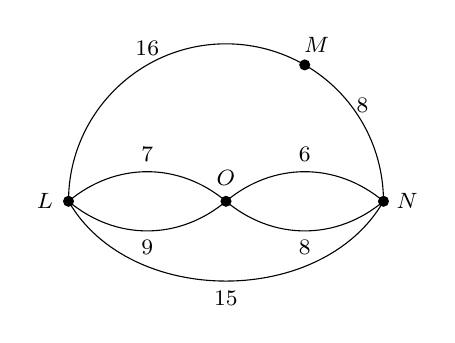
\begin{tikzpicture}[font=\footnotesize, line join=round, line cap=round, >=stealth, scale=1]
			\def\bankinh{2}
			\path (0,0) coordinate (O) (-\bankinh,0) coordinate (L) (\bankinh,0) coordinate (N) (60:\bankinh) coordinate (M);
			\draw
			(L) arc(180:60:\bankinh) node[pos=0.5, above]{$16$}
			(M) arc(60:0:\bankinh) node[pos=0.5, above]{$8$}
			(L) to[bend right=60] node[pos=0.5, below]{$15$} (N)
			(L) to[bend right=40] node[pos=0.5, below]{$9$} (O)
			(L) to[bend left=40] node[pos=0.5, above]{$7$} (O)
			(O) to[bend right=40] node[pos=0.5, below]{$8$} (N)
			(O) to[bend left=40] node[pos=0.5, above]{$6$} (N)
			;
			\foreach \x/\g in {O/90, L/180, N/0, M/60}{
			\fill (\x) circle (2pt)+(\g:0.3)node{$\x$};
			}
		\end{tikzpicture}
	\end{center}
	\par\shortans{$37$}
	\loigiai{
	Để chiều dài quãng đường là tối thiểu, cán bộ thanh tra cần xuất phát từ $L$, đi qua mỗi thị trấn $M$, $N$, $O$ đúng một lần trước khi qua lại $L$ và ưu tiên chọn con đường ngắn hơn trong hai con đường nối hai thị trấn.\\
	Ta có quãng đường tối ưu là $L\rightarrow M \rightarrow N \rightarrow O \rightarrow L$ với độ dài là $16+8+6+7=37$ km.
	}
\end{bt}

%

\begin{ex}%[Nguồn: Bộ đề minh họa Moon 2024-2025]%[1C2V1-3]
	Một con bọ di chuyển từ điểm $A$ đến điểm $B$ dọc theo các đoạn thẳng trong mạng lưới lục giác như hình bên dưới
	\begin{center}
		\begin{tikzpicture}[>=stealth,line join=round,line cap=round,font=\footnotesize,scale=1]
			\def\l{1.2}
			\newcommand{\drawhexagon}[3]{
			\begin{scope}[shift={(#1,#2)}]
				% Vẽ lục giác
				\draw (0:\l) -- (60:\l) -- (120:\l) -- (180:\l) -- (240:\l) -- (300:\l) -- cycle;
			\end{scope}
			}
			% Hàng 1
			\drawhexagon{0}{0}{}
			\draw [->] (0,1.04)--(0.1,1.04) node [above] {$1$} ;
			\draw [->] (0,-1.04)--(0.1,-1.04)node [below] {$2$};
			\draw (0,1.3) node[above] {$(C_1)$};
			% Hàng 2
			\drawhexagon{1.8}{1.04}{}
			\drawhexagon{1.8}{-1.04}{}
			\draw [->] (1.8,2.07)--(1.9,2.07) node [above] {$3$};
			\draw [<-] (1.8,0)--(1.9,0) ;
			\draw [->] (1.8,-2.08)--(1.9,-2.08)node [below] {$4$};
			\draw (1.8,2.4) node[above] {$(C_2)$};
			% Hàng 3
			\drawhexagon{3.6}{2.08}{}
			\drawhexagon{3.6}{0}{}
			\drawhexagon{3.6}{-2.08}{}
			\draw [->] (3.5,3.12)--(3.6,3.12) node [above] {$5$};
			\draw [->] (3.5,1.04)--(3.6,1.04) node [above] {$6$} ;
			\draw [->] (3.5,-1.04)--(3.6,-1.04) node [above] {$7$} ;
			\draw [->] (3.5,-3.12)--(3.6,-3.12) node [above] {$8$} ;
			\draw (3.5,3.4) node[above] {$(C_3)$};
			% Hàng 4
			\drawhexagon{5.4}{1.04}{}
			\drawhexagon{5.4}{-1.04}{}
			\draw [->] (5.2,2.07)--(5.3,2.07) node [above] {$9$};
			\draw [<-] (5.2,0)--(5.3,0) ;
			\draw [->] (5.2,-2.08)--(5.3,-2.08)node [below] {$10$};
			\draw (5.2,2.4) node[above] {$(C_4)$};
			% Hàng 5
			\drawhexagon{7.2}{0}{}
			\draw [->] (7,1.04)--(7.1,1.04) node [above] {$11$} ;
			\draw [->] (7,-1.04)--(7.1,-1.04)node [below] {$12$};
			\draw (7,1.3) node[above] {$(C_5)$};
			% Điểm A và B
			\node[fill=black,circle,inner sep=1pt,label=left:A] at (-1.2,0) {};
			\node[fill=black,circle,inner sep=1pt,label=right:B] at (8.4,0) {};
			
		\end{tikzpicture}
		
	\end{center}
	Các đoạn thẳng có dấu mũi tên chỉ được di chuyển theo hướng của mũi tên, các đọạn thẳng không có dấu mũi tên được di chuyển theo hướng tùy ý và con bọ không bao giờ di chuyển trên cùng một đoạn thẳng quá một lần. Vậy con bọ có bao nhiêu con đường khác nhau từ $A$ đến $B$?
	\shortans[1]{$100$}
	\loigiai{
	\begin{itemize}
		\item Từ $A$ có $2$ cách đến $C1$
		\begin{itemize}
		\item Từ $A$ có $1$ cách đến mũi tên số $1$;
		\item Từ $A$ có $1$ cách đến mũi tên số $2$.
	\end{itemize}
	\item Từ $C1$ có $5$ cách đến $C3$\\
	Không mất tính tổng quát giả sử đi từ $C1$ mũi tên số $1$ đến $C3$ mũi tên số $6$ hoặc mũi tên số $7$.
	\begin{itemize}
		\item Từ mũi tên số $1$ có $2$ cách để đi đến mũi tên số $6$.
		\item Từ mũi tên số $1$ có $3$ cách để đi đến mũi tên số $7$.
	\end{itemize}
	Suy ra từ $C1$ có $5$ cách đến $C3$.
	\item Từ $C3$ có $5$ cách đến $C5$\\
	Không mất tính tổng quát giả sử đi từ $C3$ mũi tên số 5 đến $C5$ mũi tên số $11$ hoặc mũi tên số $12$.
	\begin{itemize}
		\item Từ mũi tên số $5$ có $2$ cách để đi đến mũi tên số $11$.
		\item Từ mũi tên số $5$ có $3$ cách để đi đến mũi tên số $11$.
	\end{itemize}
	Suy ra từ $C3$ có $5$ cách đến $C5$.
	\item Từ $C5$ có $2$ cách đến $B$
	\begin{itemize}
		\item Từ mũi tên số $11$ có $1$ cách đến $B$.
		\item Từ mũi tên số $12$ có $1$ cách đến $B$.
	\end{itemize}
	\end{itemize}
	Vậy có $2\cdot 5\cdot 5\cdot 2 = 100$ cách đi từ $A$ đến $B$.
	}
\end{ex}

